\indent This experiment was part of a group of four experiments that commissioned the new Hall C Super High Momentum Spectrometer (SHMS) as part of the 12 GeV upgrade at JLab.
An electron beam was incident on a 10 cm long liquid deuterium target (LD2). The scattered electron and knocked-out proton were detected in coincidence
by the SHMS ans High Momentum Spectrometer (HMS), respectivly. The ``missing'' (undetected) neutron was reconstructed from momentum conservation laws.
The beam currents delivered by the accelerator ranged between 40-60 $\mu$A due to frequent beam trips at higher currents and the beam was rastered over a 2x2 mm$^{2}$ area to reduce
the effects of localized boiling on the cryogenic targets (hydrogen and deuterium). \\
\indent Both spectrometers at Hall C have similar standard detector packages, each with 1) four sets of hodoscope planes (scintillator arrays) used for triggering,
2) a pair of drift chambers used for tracking, 3) a calorimeter used for $e^{-}/\pi^{-}$ discrimination and 4) a gas \u{C}erenkov used also for $e^{-}/\pi^{-}$ and an additional
Noble Gas \u{C}erenkov used in the SHMS for $e^{-}/\pi^{+}/K^{+}$ at momenta $>$ 6 GeV/c. Due to the absence of significant background on this experiment and the low coincidence trigger rates
($\sim 1-3$ Hz) at the higher missing momentum settings, the use of additional particle identification (PID) was found to have little to no effect on the final cross section. \\
\indent We measured three missing momentum settings: $p_{r}=80,580$ and $750$ MeV/c. In the high missing momentum settings the spectrometer configuration was changed
multiple times resulting in either the spectrometer angle or momentum not being excactly the same. As a result, two separate data sets measured for the 580 MeV/c and three data sets for the 750 MeV/c setting.  
The spectrometer central settings are approximately as follows: the SHMS central angle and momentum settings were kept fixed at (12.194 deg, 8.5342 GeV/c) and the HMS central angle and momentum settings were changed from
(38.896 deg, 2.840 GeV/c) at the 80 MeV setting to (54.992 deg, 2.1925 GeV/c) and (58.391 deg, 2.0915 GeV/c) at the 580 and 750 MeV/c settings, respectively. At these kinematics, the
3-momentum transfer is $|\vec{q}| = 2.86$ GeV/c and is on the order of the final proton momentum indicating that most of the energy and momentum are transferred to the proton. As a result, the ejected proton
scatters at angles $\theta_{pq}\sim 0$, relative to the $\vec{q}$. This configuration is known as the ``parallel-kinematics'' and suppresses the process in which the neutron is struck and the proton is a spectator. \\
\indent In addition to deuteron kinematics,  $^{1}H(e,e'p)$ elastic data was also taken at kinematics close to the deuteron 80 MeV setting for cross-checks with the spectrometer acceptance model as well as for normalization purposes using the  Hall C Monte Carlo
simulation program, \texttt{SIMC}. Additional $^{1}H(e,e'p)$ data was also taken at three other kinematic settings that covered the entire SHMS momentum acceptance range and were used for spectrometer optics studies and
calibration. \\
\indent The event selection criteria was done exactly the same for the hydrogen and deuteron data. The criteria was determined by making 1) standard cuts on the spectrometer momentum fraction ($\delta$) to select a region in which the reconstruction optics
is well known, 2) an HMS collimator cut to restrict the spectrometer solid angle acceptance to events that only passed through the collimator and not by re-scattering from the edges, 3) a missing
energy cut (peak $\sim$ 2.2 MeV for the deuteron) to select true $ep$ coincidences and not events from the radiative tail, 4) a coincidence time cut to select true coincidence events and not accidentals,  5) a PID cut on the
SHMS calorimeter to select electrons and not other sources of background, mostly pions and 6) a z-vertex difference cut between the HMS and SHMS $z$ reaction vertex difference to select events that truly
originated from the same reaction vertex at the target. \\
\indent The experimental data yield was normalized by the total charge and corrected for tracking efficiencies, total live time, proton absorption and target boiling factors.
For $^{1}H(e,e'p)$, the corrected data yield was compared to SIMC using P. Bosted's proton form factor parametrization\cite{PhysRevC.51.409} to check the spectrometer acceptance
model. The data to SIMC yield ratio integrated over invariant mass $W$ was determined to be unity, so there was no need to include an overall hydrogen normalization factor. For the $^{2}H(e,e'p)n$ data,
the measured cross sections were compared to the model cross sections (incorporated as a SIMC subroutine) from calculations by J.M. Laget using the Paris potential. Variations
of up to $\sim 20 \%$ for recoil momenta up to $\sim$ 250 MeV/c were observed which are typical for this setting using the Paris potential. The 80 MeV data was also checked for reproducibility against the Hall A data.
This agreement gives us confidence on the measurements made at higher missing momentum setting for which no data exists. \\
\indent The systematic uncertainties on the measured cross sections were determined from 1) normalization and 2) kinematic uncertainties. The individual contributions from normalization uncertainties
were determined to be: tracking efficiencies ($0.40 \%$-HMS, $0.59 \%$-SHMS ), target boiling ($0.39 \%$), total live time ($3.0 \%$) and total charge ($2.0\%$)
for an overall normalization uncertainty added in quadrature of $3.7 \%$. \\
\indent The kinematic uncertainties were determined point-to-point in ($\theta_{nq}, p_{r}$) bins for each data set independently, and added in quadrature for overlapping $p_{r}$ bins
of different data sets. For $\theta_{nq}=$ 35, 45 and 75 deg (presented on this Letter) the overall kinematic uncertainty varied up to 6.5$\%$ for $p_{r}\leq1.01$ GeV/c.
The overall systematic uncertainty in the cross section was determined by the quadrature sum of the normalization and kinematic uncertainties. This results was then added in quadrature
to the statiscial uncertainty to obtain the final uncertainty in the cross section. \\
\indent The data was radiatively corrected for each bin in ($\theta_{nq}, p_{r}$) by multiplying measured cross sections to the ratio of the SIMC yield without and with radiative effects. Bin-centering
corrections were also applied by multiplying the radiative corrected cross sections to the ratio of theoretical cross sections (external to SIMC) to the average cross sections calculated from SIMC.
The theoretical calculations used in the bin-centering corrections were done by J.M. Laget using the Paris potential. \\
\indent Both experimental and theoretical reduced cross sections were extracted from the measured (or model) cross sections for each data of set independently and were averaged for overlapping bins in $p_{r}$,
where the reduced cross sections are defined as follows:
\begin{equation}
\sigma_{red} \equiv \frac{\sigma_{exp(th)}}{Kf_{rec}\sigma_{cc1}}
\label{eq:1}
\end{equation}
where $\sigma_{exp(th)}$ is the 5-fold experimental (or theoretical) differential cross section, $K$ is a kinematical factor, $f_{rec}$ is a the recoil factor that arises from the
integration over missing energy and $\sigma_{cc1}$ is the de Forest\cite{DEFOREST1983} electron-proton offshell cross section calculated from P. Bosted's form factor parametrization \cite{PhysRevC.51.409}.
Only within the PWIA, $\sigma_{red}$ can be interpreted as the proton momentum distribution inside the deuteron where most of the kinematical dependencies that arise from the
cross section have been factored out by $\sigma_{cc1}$, leaving only a dependency on $p_{r}$. \\
\begin{figure}
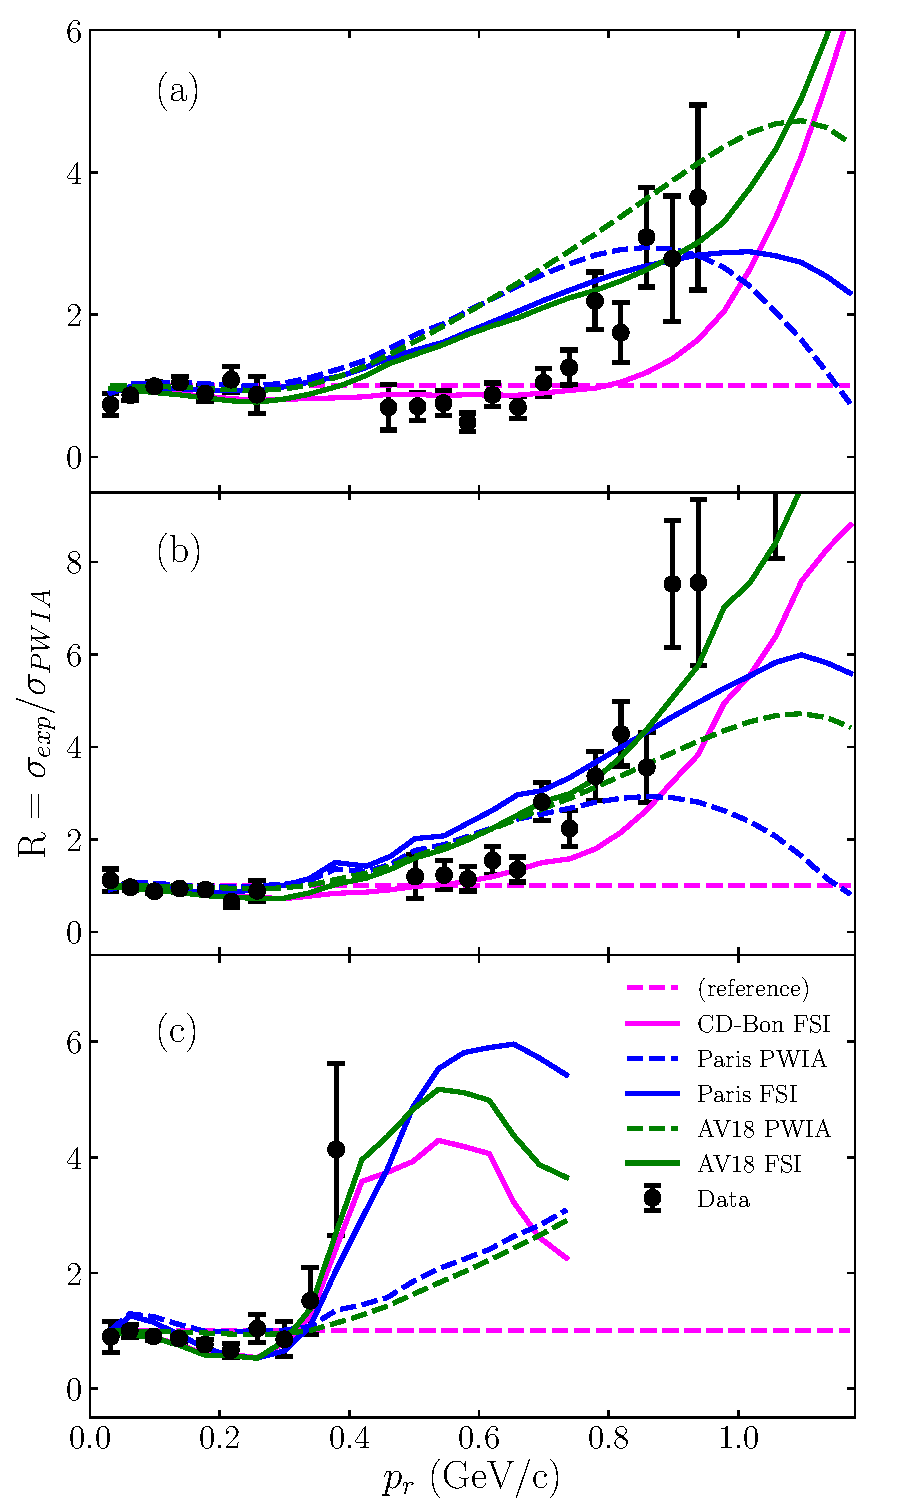
\includegraphics[scale=0.5]{../prl_plots/PRL_plot2.pdf}
\caption{The ratio R($p_{r}$) = $\sigma_{red}$/n$(p_{r})$ is shown in (a)-(c) for $\theta_{nq}=35^{o}, 45^{o}$ and $75^{o}$, respectively, each with a bin width of $\pm 5^{o}$.
                              The dashed reference (magenta) line refers to CD-Bonn momentum distribution (n$(p_{r})$) by which the data and all models are divided. }
\label{fig:fig1}
\end{figure}
\indent To quantify by how much and to what extent the data agrees with theory, the ratio of the experimental (or theoretical) reduced cross sections ($\sigma_{red}$)
to the deuteron momentum distributions (n$(p_{r})$) using the charge-dependent Bonn (CD-Bonn) potential is shown in Fig. \ref{fig:fig1}. The theoretical calculations for the
CD-Bonn and Argonne $v_{18}$ (AV18) potentials were performed by M. Sargsian and those for the Paris potential were done by J.M. Laget. For $p_{r}\lesssim 300$ MeV/c, the data is
in good agreement with all models for the neutron recoil angles shown in Fig. \ref{fig:fig1}. For $p_{r}\gtrsim 300$, at recoil angles $\theta_{nq} = 35^{o}\pm5^{o}$ [Fig. \hyperref[fig:fig1]{1(a)}],
the data is best described by the CD-Bonn curves which exhibit a reduced sensitivity to FSIs and an enhanced sensitivity to the momentum distribution with a ratio R$\sim$1 for recoil momenta
up to $\sim$ 800 MeV/c before being overwhelmed by FSIs. The data, however, is sensitive to the momentum distributions only up to $p_{r}\sim$ 750 MeV/c before transitioning to other theoretical curves
with a maximal ratio of R$\sim$3 at $p_{r}\sim$940 MeV/c due to statistical limitations. For recoil angles $\theta_{nq} = 45^{o}\pm5^{o}$ [Fig. \hyperref[fig:fig1]{1(b)}], both the data and
CD-Bonn curves show sensitivities to momentum distributions up to $p_{r}\sim$ 580 MeV/c. At $p_{r}>580$ MeV/c, FSIs become increasingly important for CD-Bonn curves, whereas the data shows
a similar behaviour as in Fig. \hyperref[fig:fig1]{1(a)} with an early rise in the ratio than predicted by the CD-Bonn FSI model. For $\theta_{nq} = 75^{o}\pm5^{o}$ [Fig. \hyperref[fig:fig1]{1(c)}], the
onset of GEA is observed beyond $p_{r}\sim$ 300 MeV/c, with a strong angular dependence of the reduced cross sections on FSIs predicted by all models and verified by data which was statistically limited
at larger recoil angles. \\
\indent Figure \ref{fig:fig2} shows the extracted experimental and theoretical reduced cross sections as a function of neutron recoil momentum, $p_{r}$ for three angular settings at 4$\leq Q^{2} \leq$5
(GeV/c)$^{2}$. The data is compared to the results from the previous Hall A experiment\cite{PhysRevLett.107.262501} at a $Q^{2}=$ 3.5 (GeV/c)$^{2}$.  The overlay of the Hall A data (cyan) in Fig. \ref{fig:fig2}
provides a continutity to the data from this experiment in the transition region from low (80 MeV/c) to high (580, 750) MeV/c missing momentum settings in which there was no data. There is also an overall good agreement between the two experiments
in the regions in which they overlap in $p_{r}$. \\
\indent At larger neutron recoil angles of $\theta_{nq}\sim75^{o}$ [Fig. \hyperref[fig:fig2]{2(c)}], the data follows the CD-Bonn PWIA (momentum distributions) up to $p_{r}\sim $100 MeV/c, and at $p_{r}\gtrsim$300 MeV/c, the FSIs become the dominat process and exhibit a
characteristic ``flattening'' (smaller falloff) with $p_{r}$. This behaviour of FSI with larger recoil angles was predicted by the GEA and was first verified by the Hall A experiment.
This experiment kinematics moves away from larger recoil angles and focuses on fowards angles at $\theta_{nq}\sim 40^{o}$ where the momentum distributions become accessible. As a result, our data at larger recoil angles
is statistically limited. \\
\indent For recoil angles at $\theta_{nq}=35^{o}$ and $45^{o}$ shown in Figs. \hyperref[fig:fig2]{2(a)}] and  \hyperref[fig:fig2]{2(b)}],  all models predict similar behaviour of the momentum distribution for recoil momenta up to $p_{r}\sim$300 MeV/c which the data verifies. At larger $p_{r}$,
however, the momentum distributions become increasingly sensitive to the NN potentials, mainly a difference between the CD-Bonn and either the Paris or AV18 is observed. \\
\indent In Fig. \hyperref[fig:fig2]{2(a)} for example, the data clearly favors the CD-Bonn momentum distributions between recoil momenta of $300\lesssim p_{r}\lesssim750$ MeV/c before transitioning to the Paris/AV18 potentials which is a behaviour that is not well described by any of the models.
For recoil angles in Fig. \hyperref[fig:fig2]{2(b)}, a similar behaviour can be observed, as the data is sensitive to the CD-Bonn momentum distributions but only up to $p_{r}\sim 580$ MeV/c as FSIs start to dominate at lower $p_{r}$
as opposed to Fig. \hyperref[fig:fig2]{2(a)}. For $p_{r}>580$ MeV/c, the data again exhibits a behaviour at the high momentum tails which either the CD-Bonn, Paris or AV18 potentials are unable to describe.
\onecolumngrid

\begin{figure}[bh!]
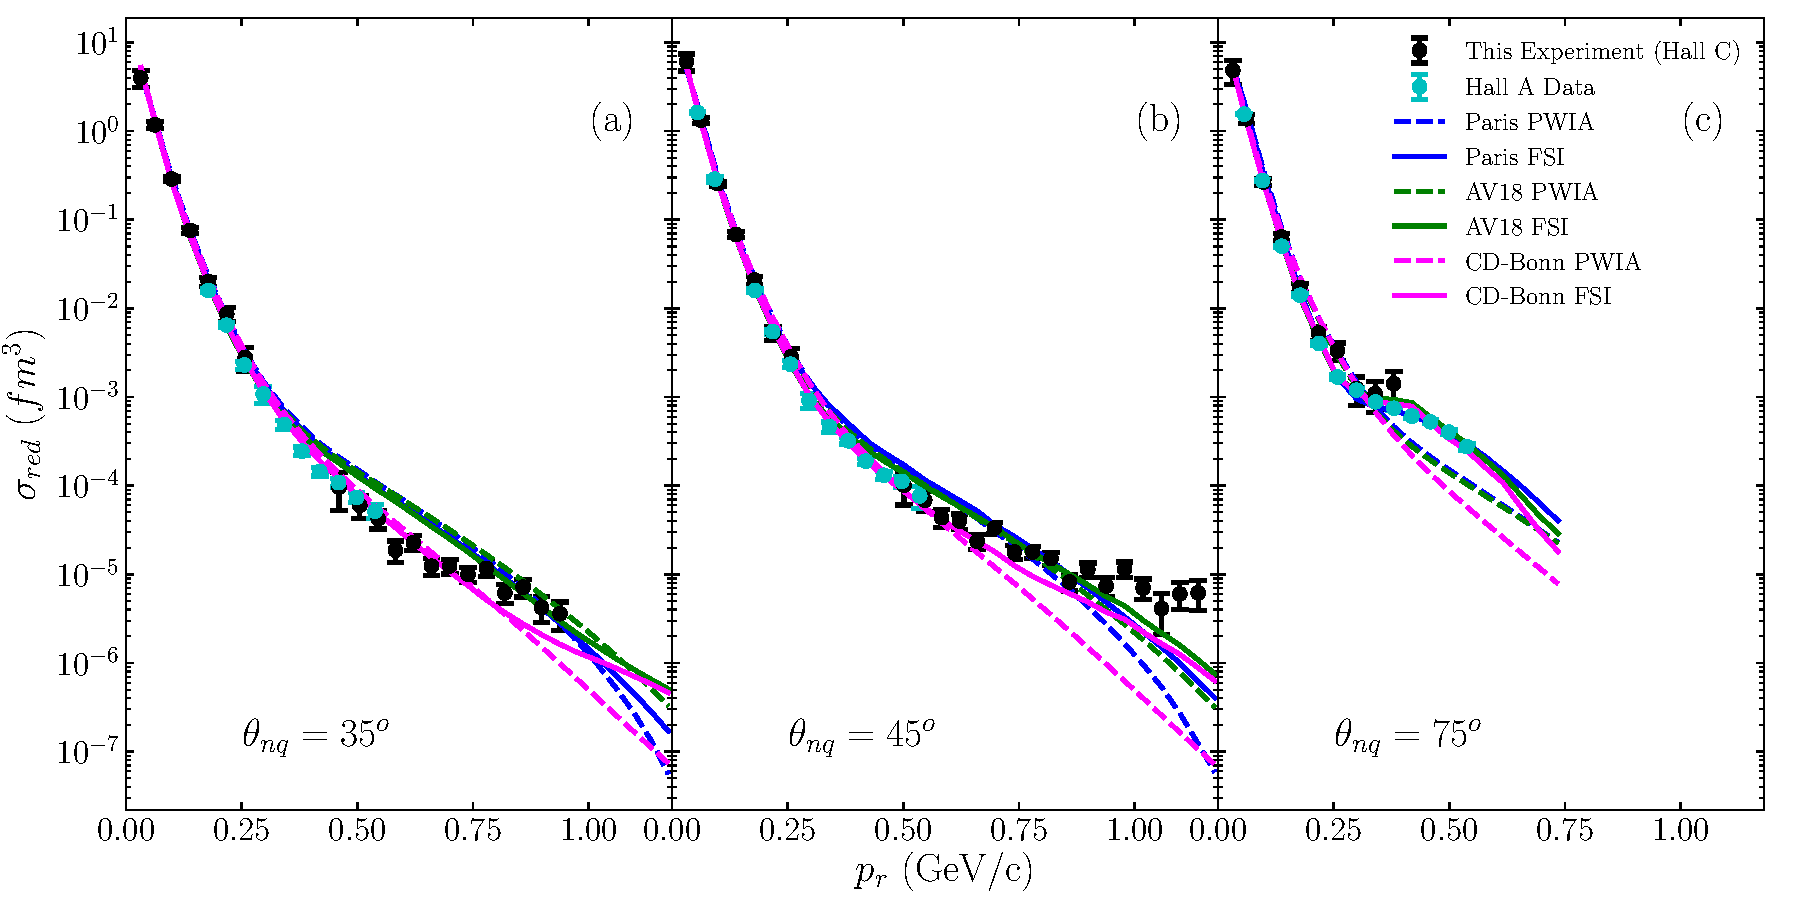
\includegraphics[scale=0.5]{../prl_plots/PRL_plot1.pdf}
\caption{The reduced cross section $\sigma_{red}(p_{r})$ as a function of neutron recoil momentum $p_{r}$ is shown in (a)-(c) for recoil angles \\  $\theta_{nq}=35^{o}, 45^{o}$ and $75^{o}$, respectively,
with a bin width of $\pm 5^{o}$. The data is compared to the previous Hall A experiment results as well as the Paris, AV18 and CD-Bonn theoretical reduced cross sections.}
\label{fig:fig2}
\end{figure}

\twocolumngrid
\indent In summary, this commissioning experiment extends the previous Hall A cross section measurements on the $^{2}H(e,e'p)n$ reaction to 
unprecedented large $Q^{2}$ and very high neutron recoil momenta at kinematics that enhances the high momentum components of the deuteron wavefunctions
while suppressing long-range processes such as MECs or ICs. FSIs have also been largely suppressed by selecting a kinematic window found in the previous Hall A 
experiment where FSIs were found to be reduced and independent of missing momentum at recoil angles $35^{o}\leq\theta_{nq}\leq45^{o}$. This experiment took advantage
of that kinematic window and extended the cross section measurements beyond $p_{r}\sim$500 MeV/c. The experimental reduced cross sections were extracted and found to
be best described by the CD-Bonn potential with sensitivity to the CD-Bonn momentum distributions up to $p_{r}\sim580$ and $750$ MeV/c for $\theta_{nq}\sim45^{o}$ and $35^{o}$,
respectively before the data transitioning to other theoretical models, which is a behavior that was not predicted by any of the models. We conclude that these results although
very interesting, does not have the sufficient statistics and the required number of high missing momentum settings to make a definitive argument about the underlying physics observed.


%high momentum components of the deuteron wavefunction by suppressing other reaction mechanisms such as MECs or ICs 


